\documentclass[tikz,border=8pt]{standalone}
% Shared look for every TikZ diagram. Load with \input{../../tools/tikz-style.tex}
\usepackage[T1]{fontenc}
\usepackage{lmodern}
\renewcommand{\sfdefault}{lmr}  % diagrams use the same serif as the text
\usetikzlibrary{arrows.meta, positioning, shapes.geometric, calc, fit, backgrounds}
\definecolor{cblue}{HTML}{4C78A8}
\definecolor{corange}{HTML}{F58518}
\definecolor{cgreen}{HTML}{54A24B}
\definecolor{cred}{HTML}{E45756}
\definecolor{cpurple}{HTML}{B279A2}
\definecolor{cgrey}{HTML}{6B6B6B}
\tikzset{
  every picture/.style={font=\sffamily, line width=1.2pt},
  box/.style={draw=#1, fill=#1!12, rounded corners=4pt, align=center, inner sep=7pt, minimum height=1.1cm},
  box/.default=cgrey,
  arrow/.style={-{Stealth[length=3mm]}, draw=cgrey, line width=1.4pt},
  title/.style={font=\sffamily\bfseries\Large},
  note/.style={font=\sffamily\small, text=cgrey, align=center},
}
\AtBeginDocument{\hyphenpenalty=10000 \exhyphenpenalty=10000}

\tikzset{cell/.style={draw=#1, fill=#1!10, minimum height=0.75cm, inner xsep=6pt},
  piece/.style={draw=cgrey, fill=white, rounded corners=2pt, minimum height=0.65cm, inner xsep=4pt}}
\begin{document}
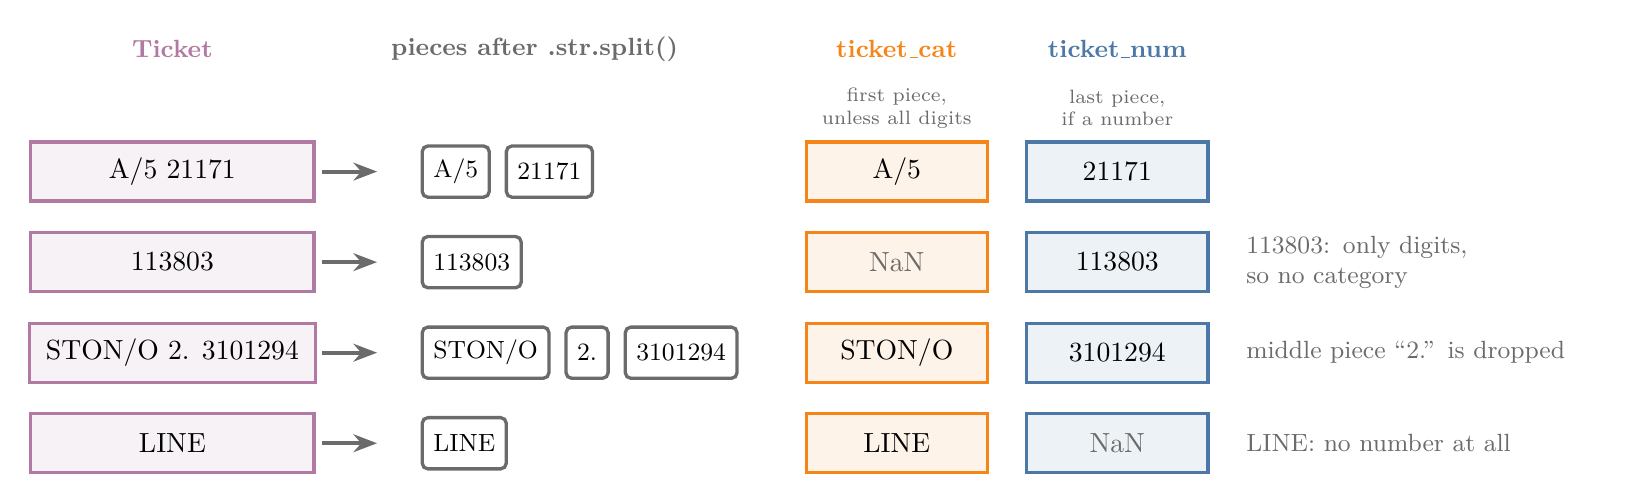
\begin{tikzpicture}[x=1cm, y=1.15cm]
  % headers
  \foreach \x/\t/\c in {0/Ticket/cpurple, 4.6/{pieces after .str.split()}/cgrey, 9.2/ticket\_cat/corange, 12/ticket\_num/cblue}
    \node[font=\sffamily\bfseries\small, text=\c] at (\x,0.85) {\t};
  \node[note, font=\sffamily\scriptsize] at (9.2,0.2) {first piece,\\ unless all digits};
  \node[note, font=\sffamily\scriptsize] at (12,0.2) {last piece,\\ if a number};
  % rows: ticket / pieces (first,middle,last) / cat / num
  \foreach \y/\t/\p/\cat/\num [count=\i] in {
      -0.5/{A/5 21171}/{A/5,21171}/{A/5}/21171,
      -1.5/{113803}/{113803}/\textcolor{cgrey}{NaN}/113803,
      -2.5/{STON/O 2. 3101294}/{STON/O,2.,3101294}/{STON/O}/3101294,
      -3.5/{LINE}/{LINE}/{LINE}/\textcolor{cgrey}{NaN}} {
    \node[cell=cpurple, minimum width=3.6cm] at (0,\y) {\t};
    \draw[arrow] (1.9,\y) -- (2.6,\y);
    \node[anchor=west] (p\i) at (2.7,\y) {};
    \def\last{p\i}
    \foreach \q in \p {
      \node[piece, anchor=west, right=5pt of \last] (cur) {\small\q};
      \global\let\last\relax \xdef\last{cur}
    }
    \node[cell=corange, minimum width=2.3cm] at (9.2,\y) {\cat};
    \node[cell=cblue, minimum width=2.3cm] at (12,\y) {\num};
  }
  \node[note, anchor=west, text width=4.6cm, align=left] at (13.5,-1.5) {113803: only digits,\\ so no category};
  \node[note, anchor=west, text width=4.6cm, align=left] at (13.5,-2.5) {middle piece ``2.'' is dropped};
  \node[note, anchor=west, text width=4.6cm, align=left] at (13.5,-3.5) {LINE: no number at all};
\end{tikzpicture}
\end{document}
